\documentclass{article}
\usepackage[utf8]{inputenc} %кодировка
\usepackage[T2A]{fontenc}
\usepackage[english,russian]{babel} %русификатор 
\usepackage{mathtools} %библиотека матеши
\usepackage[left=1cm,right=1cm,top=2cm,bottom=2cm,bindingoffset=0cm]{geometry} %изменение отступов на листе
\usepackage{amsmath}
\usepackage{graphicx} %библиотека для графики и картинок
\graphicspath{}
\DeclareGraphicsExtensions{.pdf,.png,.jpg}
\usepackage{subcaption}
\usepackage{pgfplots}
\usepackage{float}
\usepackage{listings}
\usepackage{tikz}


\lstset{
    numbers=left,            % Нумерация строк слева
    numberstyle=\tiny,       % Размер шрифта для номеров строк
    stepnumber=1,            % Нумеровать каждую строку
    numbersep=5pt,           % Расстояние между номерами и кодом
    backgroundcolor=\color{white},  % Цвет фона
    showspaces=false,        % Не показывать пробелы
    showstringspaces=false,  % Не показывать пробелы в строках
    showtabs=false,          % Не показывать табуляцию
    frame=single,            % Рамка вокруг кода
    tabsize=2,               % Размер табуляции
    breaklines=true,         % Автоматический перенос строк
    breakatwhitespace=true   % Переносить строки только по пробелам
}

\begin{document}
% НАЧАЛО ТИТУЛЬНОГО ЛИСТА
\begin{center}
    \Large
    Федеральное государственное автономное \\
    образовательное учреждение высшего образования \\ 
    «Научно-образовательная корпорация ИТМО»\\
    \vspace{0.5cm}
    \large
    Факультет программной инженерии и компьютерной техники \\
    Направление подготовки 09.03.04 Программная инженерия \\
    \vspace{1cm}
    \Large
    \textbf{Отчёт по лабораторной работе №4} \\
        По дисциплине «Системы ввода-вывода» ( семестр 6)\\
    \large
    \vspace{8cm}

    \begin{minipage}{.33\textwidth}
    \end{minipage}
    \hfill
    \begin{minipage}{.4\textwidth}
    
        \textbf{Студент}: \vspace{.1cm} \\
        \ Дениченко Александр P3312\\
        \ Разинкин Александр P3307\\
        \ Балин Артём P3312\\
        \textbf{Практик}:  \\
        \ Табунщик Сергей Михайлович
    \end{minipage}
    \vfill
Санкт-Петербург\\ 2025 г.
\end{center}
\pagestyle{empty}
% КОНЕЦ ТИТУЛЬНОГО ЛИСТА 
\newpage
\pagestyle{plain}

\section*{Цель}
Изучение протоколов передачи данных между устройствами.
Познакомится с принципами обмена данными между
устройствами, алгоритмами обмена и форматами передачи данных на
примере интерфейсов I2C, SPI, 1-Wire.
\section{Задачи}
.

1. Написать программу для микроконтроллера Atmega328, принимающую и отправляющую
пакеты по интерфейсу UART в соответствии с обозначенным форматом пакета. Драйвер UART
должен быть реализован с использованием операций ввода/вывода в регистры аппаратного
контроллера UART.

2. Контроллер должен принимать данные с ПК, проверять их на корректность и отправлять
обратно корректные пакеты. Если пакет пришел с ошибкой, то он отбрасывается.

3. Контроллер должен раз в секунду передавать данные с датчика, указанного в варианте
задания.

4. Написать клиентскую программу на ПК для приема и отправки пакетов к микроконтроллеру
по интерфейсу UART, моделирующей как корректную отправку пакетов, так и случаи с
ошибками: неправильная длина, отсутствие синхробайта, недостаточное количество данных.

5. Подключить микроконтроллер к ПК и протестировать работоспособность написанных
программ

6. Снять осциллограмму передачи любого пакета по интерфейсу UART

7. Оформить отчет по работе в электронном формате

\section{Вариант 2}

Датчик BMP280, SPI температура и давление -- Скорость UART 38400 -- Четность odd parity -- Кол-во
стоповых бит 2

\section{Выполнение}

\begin{lstlisting}[caption={sketch}, label={lst:example}]
  #include <Wire.h>
  #include <Adafruit_BMP280.h>
  
  #define BMP_CS 10
  
  Adafruit_BMP280 bmp(BMP_CS);
  
  void UART_Init();
  void UART_Transmit(char data);
  void UART_SendString_P(const char* str);
  void UART_SendInt(int num);
  void UART_SendFloat(float num);
  
  void setup() {
      UART_Init();
      delay(100);
  
      unsigned status;
      status = bmp.begin();
      if (!status) {
          UART_SendString_P(PSTR("Could not find BMP280 sensor!\r\n"));
          while(1);
      }
  
      bmp.setSampling(Adafruit_BMP280::MODE_NORMAL,
                      Adafruit_BMP280::SAMPLING_X2,
                      Adafruit_BMP280::SAMPLING_X16,
                      Adafruit_BMP280::FILTER_X16,
                      Adafruit_BMP280::STANDBY_MS_500);
  }
  
  void loop() {
      UART_SendString_P(PSTR("Temperature = "));
      UART_SendFloat(bmp.readTemperature());
      UART_SendString_P(PSTR(" *C\r\n"));
  
      UART_SendString_P(PSTR("Pressure = "));
      UART_SendLong((long)bmp.readPressure());
      UART_SendString_P(PSTR(" Pa\r\n\r\n"));
  
      delay(2000);
  }
  
  void UART_Init() {
      uint16_t ubrr = F_CPU / 16 / 9600 - 1;
      UBRR0H = (uint8_t)(ubrr >> 8);
      UBRR0L = (uint8_t)ubrr;
      UCSR0B = (1 << TXEN0);
      UCSR0C = (1 << UCSZ01) | (1 << UCSZ00);
  }
  
  void UART_Transmit(char data) {
      while (!(UCSR0A & (1 << UDRE0)));
      UDR0 = data;
  }
  
  void UART_SendString_P(const char* str) {
      char c;
      while ((c = pgm_read_byte(str++))) {
          UART_Transmit(c);
      }
  }
  
  void UART_SendInt(int num) {
      if (num < 0) {
          UART_Transmit('-');
          num = -num;
      }
      char buffer[10];
      int i = 0;
      
      do {
          buffer[i++] = num % 10 + '0';
          num /= 10;
      } while (num > 0);
      
      while (i > 0) {
          UART_Transmit(buffer[--i]);
      }
  }
  void UART_SendLong(long num) {
      if (num < 0) {
          UART_Transmit('-');
          num = -num;
      }
      char buffer[12];
      int i = 0;
      
      do {
          buffer[i++] = num % 10 + '0';
          num /= 10;
      } while (num > 0);
      
      while (i > 0) {
          UART_Transmit(buffer[--i]);
      }
  }
  
  void UART_SendFloat(float num) {
      if (num < 0) {
          UART_Transmit('-');
          num = -num;
      }
      
      long integerPart = (long)num;
      UART_SendLong(integerPart);
      UART_Transmit('.');
      
      int decimalPart = (int)((num - integerPart) * 100 + 0.5);
      if (decimalPart < 10) UART_Transmit('0');
      UART_SendInt(decimalPart);
  }
\end{lstlisting}

\section{+ client mode}

\begin{lstlisting}[caption={update ino}, label={lst:example}]
  /**
  * UART communication program for Atmega328
  * - Receives packets with format: [SYNC(0x5A)][LENGTH][DATA][CHECKSUM]
  * - Validates packets and echoes back valid ones
  * - Sends sensor data every second
  * - Uses odd parity and 2 stop bits
  */
 
 // Constants
 #define F_CPU 16000000UL  // 16 MHz clock
 #define BAUD 38400        // Baud rate
 #define SYNC_BYTE 0x5A    // Sync byte for packet validation
 
 // Calculated UBRR value for UART
 #define UBRR_VAL ((F_CPU / (16UL * BAUD)) - 1)
 
 // Timer constants for 1-second interval
 #define TIMER1_PRESCALER 256
 #define TIMER1_COMPARE_VALUE (F_CPU / TIMER1_PRESCALER) // For 1 second
 
 // Buffer sizes
 #define MAX_PACKET_SIZE 64
 #define MAX_DATA_SIZE (MAX_PACKET_SIZE - 3) // Subtract sync, length, checksum
 
 // Packet parsing states
 typedef enum {
   STATE_WAITING_SYNC,
   STATE_READING_LENGTH,
   STATE_READING_DATA,
   STATE_READING_CHECKSUM
 } PacketState;
 
 // Global variables
 volatile uint8_t rxBuffer[MAX_PACKET_SIZE]; // Buffer for incoming data
 volatile uint8_t dataBuffer[MAX_DATA_SIZE]; // Buffer for packet data
 volatile uint8_t dataLength = 0;           // Length of current data
 volatile PacketState state = STATE_WAITING_SYNC;
 volatile uint8_t bytesRead = 0;            // Bytes read in current state
 volatile uint8_t sendSensorData = 0;       // Flag for sending sensor data
 
 // Function prototypes
 void uartInit(void);
 void timerInit(void);
 uint8_t calculateChecksum(uint8_t *data, uint8_t length);
 void sendPacket(uint8_t *data, uint8_t length);
 uint16_t readSensor(void);
 
 void setup() {
   // Initialize UART with direct register access
   uartInit();
   
   // Initialize timer for 1-second sensor data transmission
   timerInit();
   
   // Initialize ADC for sensor readings
   // Enable ADC with prescaler 128 (16MHz/128 = 125kHz)
   ADCSRA = (1 << ADEN) | (1 << ADPS2) | (1 << ADPS1) | (1 << ADPS0);
   ADMUX = (1 << REFS0); // Use AVCC as reference, ADC0 as input
 }
 
 void loop() {
   // Check if it's time to send sensor data
   if (sendSensorData) {
     sendSensorData = 0;
     
     // Read from sensor
     uint16_t sensorValue = readSensor();
     
     // Prepare packet with sensor data
     uint8_t sensorPacket[3]; // 2 bytes for the sensor value + 1 for packet type
     sensorPacket[0] = 0x01;  // Packet type: Sensor data
     sensorPacket[1] = (uint8_t)(sensorValue >> 8);  // High byte
     sensorPacket[2] = (uint8_t)(sensorValue & 0xFF); // Low byte
     
     // Send the packet
     sendPacket(sensorPacket, sizeof(sensorPacket));
   }
 }
 
 // Initialize UART with direct register access
 void uartInit(void) {
   // Set baud rate
   UBRR0H = (uint8_t)(UBRR_VAL >> 8);
   UBRR0L = (uint8_t)UBRR_VAL;
   
   // Enable transmitter and receiver, and receive interrupt
   UCSR0B = (1 << RXEN0) | (1 << TXEN0) | (1 << RXCIE0);
   
   // Set frame format: 8 data bits, odd parity, 2 stop bits
   UCSR0C = (1 << UCSZ01) | (1 << UCSZ00) | // 8-bit data
            (1 << UPM01) | (1 << UPM00) |    // Odd parity
            (1 << USBS0);                    // 2 stop bits
 }
 
 // Initialize timer for 1-second intervals
 void timerInit(void) {
   // Set timer1 to CTC mode
   TCCR1A = 0;
   TCCR1B = (1 << WGM12) | (1 << CS12); // CTC mode, prescaler 256
   
   // Set compare value for 1 second
   OCR1A = TIMER1_COMPARE_VALUE;
   
   // Enable timer compare interrupt
   TIMSK1 = (1 << OCIE1A);
   
   // Enable global interrupts
   sei();
 }
 // UART receive interrupt
ISR(USART_RX_vect) {
  // Read received byte
  uint8_t receivedByte = UDR0;
  
  // Check for UART errors (frame error, parity error, data overrun)
  uint8_t error = UCSR0A & ((1 << FE0) | (1 << UPE0) | (1 << DOR0));
  
  if (error) {
    // Reset state machine if there's an error
    state = STATE_WAITING_SYNC;
    return;
  }
  
  // Process based on current state
  switch (state) {
    case STATE_WAITING_SYNC:
      if (receivedByte == SYNC_BYTE) {
        rxBuffer[0] = SYNC_BYTE;
        state = STATE_READING_LENGTH;
      }
      break;
      
    case STATE_READING_LENGTH:
      dataLength = receivedByte;
      rxBuffer[1] = dataLength;
      
      if (dataLength > MAX_DATA_SIZE) {
        // Invalid length, reset state machine
        state = STATE_WAITING_SYNC;
      } else {
        bytesRead = 0;
        state = STATE_READING_DATA;
      }
      break;
      
    case STATE_READING_DATA:
      // Store data byte
      dataBuffer[bytesRead] = receivedByte;
      rxBuffer[2 + bytesRead] = receivedByte;
      bytesRead++;
      
      if (bytesRead >= dataLength) {
        state = STATE_READING_CHECKSUM;
      }
      break;
      
    case STATE_READING_CHECKSUM:
      // Store and check checksum
      uint8_t receivedChecksum = receivedByte;
      uint8_t calculatedChecksum = calculateChecksum(dataBuffer, dataLength);
      
      if (receivedChecksum == calculatedChecksum) {
        // Valid packet received, echo it back
        sendPacket(dataBuffer, dataLength);
      }
      
      // Reset for next packet
      state = STATE_WAITING_SYNC;
      break;
  }
}

// Timer1 compare interrupt for periodic sensor reading
ISR(TIMER1_COMPA_vect) {
  sendSensorData = 1;
}

// Calculate checksum (XOR of all data bytes)
uint8_t calculateChecksum(uint8_t *data, uint8_t length) {
  uint8_t checksum = 0;
  for (uint8_t i = 0; i < length; i++) {
    checksum ^= data[i];
  }
  return checksum;
}

// Send a packet with the standard format
void sendPacket(uint8_t *data, uint8_t length) {
  // Wait until transmit buffer is empty
  while (!(UCSR0A & (1 << UDRE0)));
  UDR0 = SYNC_BYTE;
  
  // Wait until transmit buffer is empty
  while (!(UCSR0A & (1 << UDRE0)));
  UDR0 = length;
  
  // Send data bytes
  for (uint8_t i = 0; i < length; i++) {
    // Wait until transmit buffer is empty
    while (!(UCSR0A & (1 << UDRE0)));
    UDR0 = data[i];
  }
  
  // Send checksum
  uint8_t checksum = calculateChecksum(data, length);
  while (!(UCSR0A & (1 << UDRE0)));
  UDR0 = checksum;
}

// Read sensor data from ADC
uint16_t readSensor(void) {
  // Start conversion
  ADCSRA |= (1 << ADSC);
  
  // Wait for conversion to complete
  while (ADCSRA & (1 << ADSC));
  
  // Return result
  return ADC;
}
\end{lstlisting}

\begin{lstlisting}[caption={client}, label={lst:example}]
  import serial
  import time
  import random
  import struct
  
  class UARTClient:
      # Standard packet format:
      # [SYNC_BYTE(1)] [LENGTH(1)] [DATA(n)] [CHECKSUM(1)]
      SYNC_BYTE = 0x5A
  
      def init(self, port='COM5', baudrate=38400):
          self.ser = serial.Serial(
              port=port, 
              baudrate=baudrate, 
              bytesize=serial.EIGHTBITS,
              parity=serial.PARITY_ODD,  # Odd parity
              stopbits=serial.STOPBITS_TWO,  # 2 stop bits
              timeout=1
          )
          if not self.ser.is_open:
              self.ser.open()
          print(f"Connected to {port} at {baudrate} baud, odd parity, 2 stop bits")
          time.sleep(2)  # Give time for Arduino to reset
  
      def del(self):
          if hasattr(self, 'ser') and self.ser.is_open:
              self.ser.close()
              print("Serial port closed")
  
      def calculate_checksum(self, data):
          """Calculate simple XOR checksum of all data bytes"""
          checksum = 0
          for byte in data:
              checksum ^= byte
          return checksum
  
      def send_packet(self, data, corrupt_type=None):
          """
          Send a packet with optional corruption for testing
          
          corrupt_type options:
          - None: Send normal, valid packet
          - 'no_sync': Omit the sync byte
          - 'wrong_length': Set incorrect length
          - 'wrong_checksum': Use incorrect checksum
          - 'short_data': Send less data than specified in length
          """
          # Prepare basic packet
          packet = bytearray()
          
          # Add sync byte (unless corrupting)
          if corrupt_type != 'no_sync':
              packet.append(self.SYNC_BYTE)
          else:
              packet.append(0x00)  # Invalid sync byte
              
          # Add length byte
          if corrupt_type == 'wrong_length':
              packet.append(len(data) + 2)  # Incorrect length
          else:
              packet.append(len(data))  # Correct length
              
          # Add data
          if corrupt_type == 'short_data':
              # Only add half the data
              packet.extend(data[:len(data)//2])
          else:
              packet.extend(data)
              
          # Add checksum
          if corrupt_type == 'wrong_checksum':
              packet.append((self.calculate_checksum(data) + 1) % 256)  # Incorrect checksum
          else:
              packet.append(self.calculate_checksum(data))  # Correct checksum
              
          # Send the packet
          self.ser.write(packet)
          
          # Print what was sent
          print(f"Sent: {' '.join([f'{b:02X}' for b in packet])}")
          
          return len(packet)
          def receive_packet(self, timeout=1.0):
          """Receive and parse response packet with timeout"""
          start_time = time.time()
          
          # Wait for sync byte
          while (time.time() - start_time) < timeout:
              if self.ser.in_waiting > 0:
                  sync = self.ser.read(1)
                  if sync and sync[0] == self.SYNC_BYTE:
                      break
          else:
              print("Timeout waiting for sync byte")
              return None
              
          # Read length
          if self.ser.in_waiting < 1:
              time.sleep(0.1)  # Small delay to ensure data arrival
              if self.ser.in_waiting < 1:
                  print("Failed to receive length byte")
                  return None
                  
          length = self.ser.read(1)[0]
          
          # Read data
          data = bytearray()
          if length > 0:
              wait_time = 0
              while len(data) < length and wait_time < timeout:
                  if self.ser.in_waiting > 0:
                      data.extend(self.ser.read(min(length - len(data), self.ser.in_waiting)))
                  else:
                      time.sleep(0.01)
                      wait_time += 0.01
                      
              if len(data) < length:
                  print(f"Incomplete data: received {len(data)}/{length} bytes")
                  return None
                  
          # Read checksum
          if self.ser.in_waiting < 1:
              time.sleep(0.1)
              if self.ser.in_waiting < 1:
                  print("Failed to receive checksum byte")
                  return None
                  
          checksum = self.ser.read(1)[0]
          
          # Verify checksum
          calculated_checksum = self.calculate_checksum(data)
          if checksum != calculated_checksum:
              print(f"Checksum error: received {checksum:02X}, calculated {calculated_checksum:02X}")
              return None
              
          # Packet received successfully
          packet = bytearray([self.SYNC_BYTE, length]) + data + bytearray([checksum])
          print(f"Received: {' '.join([f'{b:02X}' for b in packet])}")
          
          return data
  
      def test_communication(self):
          """Run a series of tests including normal and corrupted packets"""
          tests = [
              ("Normal valid packet", None),
              ("Missing sync byte", "no_sync"),
              ("Incorrect length", "wrong_length"),
              ("Incorrect checksum", "wrong_checksum"),
              ("Incomplete data", "short_data")
          ]
          
          for test_name, corruption in tests:
              print(f"\n=== Testing: {test_name} ===")
              # Create random test data (3-10 bytes)
              data = bytearray([random.randint(0, 255) for _ in range(random.randint(3, 10))])
              print(f"Test data: {' '.join([f'{b:02X}' for b in data])}")
              
              # Send the packet with specified corruption
              self.send_packet(data, corruption)
              time.sleep(0.5)
              
              # Try to receive response
              response = self.receive_packet()
              if response:
                  print(f"Response received: {' '.join([f'{b:02X}' for b in response])}")
              else:
                  print("No valid response received (as expected for corrupted packets)")
              
              time.sleep(1)  # Pause between tests
              def receive_packet(self, timeout=1.0):
              """Receive and parse response packet with timeout"""
              start_time = time.time()
              
              # Wait for sync byte
              while (time.time() - start_time) < timeout:
                  if self.ser.in_waiting > 0:
                      sync = self.ser.read(1)
                      if sync and sync[0] == self.SYNC_BYTE:
                          break
              else:
                  print("Timeout waiting for sync byte")
                  return None
                  
              # Read length
              if self.ser.in_waiting < 1:
                  time.sleep(0.1)  # Small delay to ensure data arrival
                  if self.ser.in_waiting < 1:
                      print("Failed to receive length byte")
                      return None
                      
              length = self.ser.read(1)[0]
              
              # Read data
              data = bytearray()
              if length > 0:
                  wait_time = 0
                  while len(data) < length and wait_time < timeout:
                      if self.ser.in_waiting > 0:
                          data.extend(self.ser.read(min(length - len(data), self.ser.in_waiting)))
                      else:
                          time.sleep(0.01)
                          wait_time += 0.01
                          
                  if len(data) < length:
                      print(f"Incomplete data: received {len(data)}/{length} bytes")
                      return None
                      
              # Read checksum
              if self.ser.in_waiting < 1:
                  time.sleep(0.1)
                  if self.ser.in_waiting < 1:
                      print("Failed to receive checksum byte")
                      return None
                      
              checksum = self.ser.read(1)[0]
              
              # Verify checksum
              calculated_checksum = self.calculate_checksum(data)
              if checksum != calculated_checksum:
                  print(f"Checksum error: received {checksum:02X}, calculated {calculated_checksum:02X}")
                  return None
                  
              # Packet received successfully
              packet = bytearray([self.SYNC_BYTE, length]) + data + bytearray([checksum])
              print(f"Received: {' '.join([f'{b:02X}' for b in packet])}")
              
              return data
      
      def test_communication(self):
          """Run a series of tests including normal and corrupted packets"""
          tests = [
              ("Normal valid packet", None),
              ("Missing sync byte", "no_sync"),
              ("Incorrect length", "wrong_length"),
              ("Incorrect checksum", "wrong_checksum"),
              ("Incomplete data", "short_data")
          ]
          
          for test_name, corruption in tests:
              print(f"\n=== Testing: {test_name} ===")
              # Create random test data (3-10 bytes)
              data = bytearray([random.randint(0, 255) for _ in range(random.randint(3, 10))])
              print(f"Test data: {' '.join([f'{b:02X}' for b in data])}")
              
              # Send the packet with specified corruption
              self.send_packet(data, corruption)
              time.sleep(0.5)
              
              # Try to receive response
              response = self.receive_packet()
              if response:
                  print(f"Response received: {' '.join([f'{b:02X}' for b in response])}")
              else:
                  print("No valid response received (as expected for corrupted packets)")
              
              time.sleep(1)  # Pause between tests'
              if name == "main":
              try:
                  client = UARTClient()
                  
                  print("\n== Running communication tests with various corruptions ==")
                  client.test_communication()
                  
                  print("\n== Starting regular communication mode ==")
                  while True:
                      # Send a normal packet with random data
                      data = bytearray([random.randint(0, 255) for _ in range(random.randint(3, 8))])
                      print(f"\nSending data: {' '.join([f'{b:02X}' for b in data])}")
                      client.send_packet(data)
                      
                      # Receive response from microcontroller
                      response = client.receive_packet()
                      if response:
                          print(f"Response received: {' '.join([f'{b:02X}' for b in response])}")
                          
                      # Wait for the 1-second sensor data that should come from microcontroller
                      print("Waiting for periodic sensor data...")
                      sensor_data = client.receive_packet(timeout=1.5)
                      if sensor_data:
                          print(f"Sensor data received: {' '.join([f'{b:02X}' for b in sensor_data])}")
                      
                      time.sleep(2)
                      
              except KeyboardInterrupt:
                  print("\nProgram terminated by user")
              except serial.SerialException as e:
                  print(f"Serial error: {e}")
                  print("Make sure the COM5 port is available and not in use by another program")
\end{lstlisting}

\section{Logic 2}

\begin{center}
  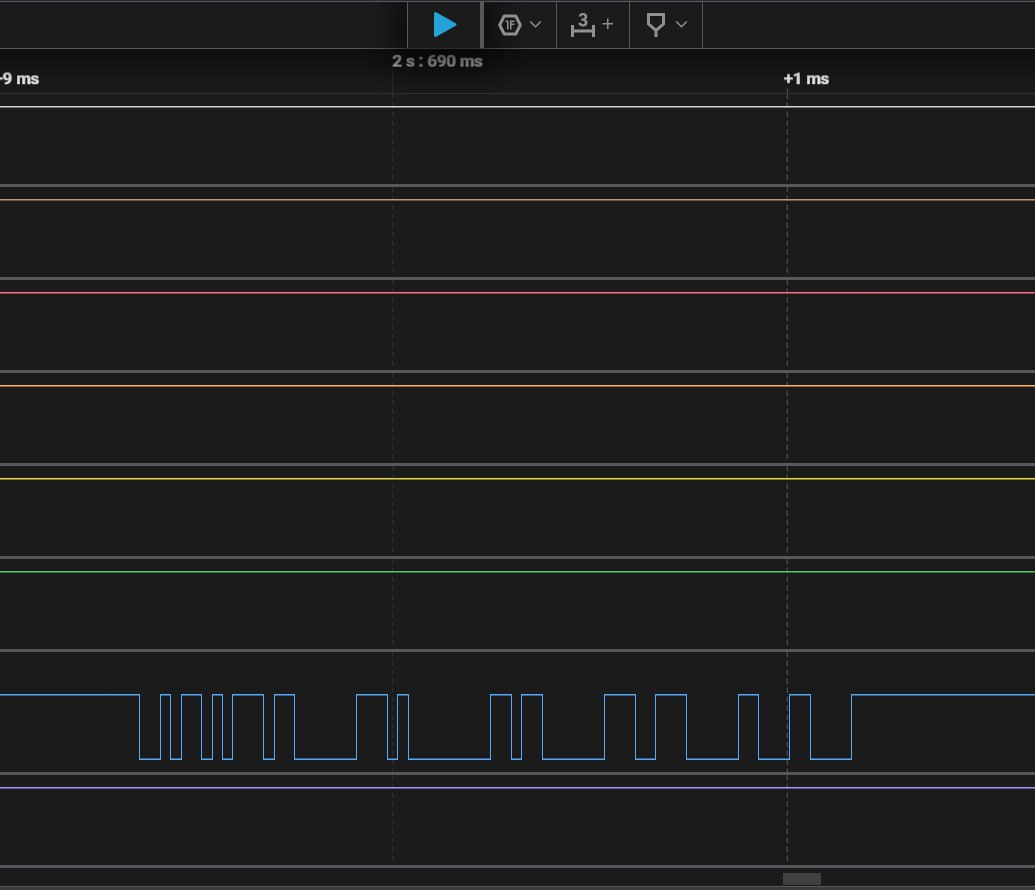
\includegraphics[width=.9\textwidth]{any}
\end{center}

\section{Example}

\begin{center}
  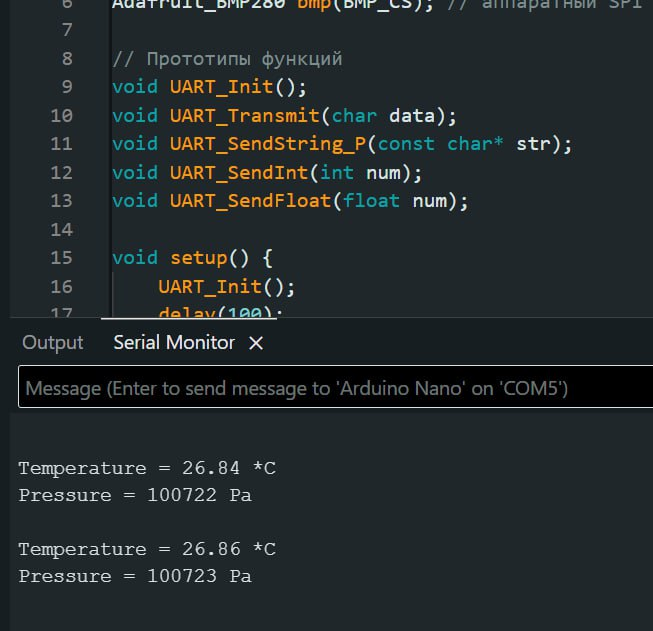
\includegraphics[width=.9\textwidth]{exmpl}
\end{center}

\section{Client out}

\begin{center}
  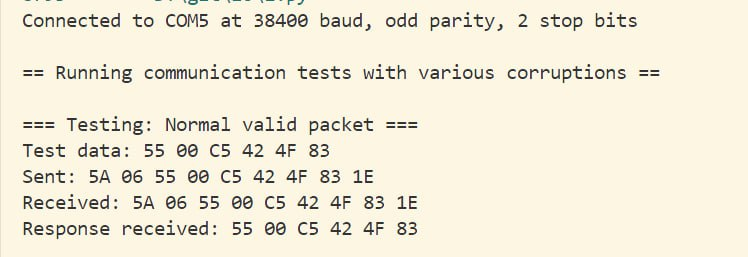
\includegraphics[width=.9\textwidth]{image}
\end{center}

\end{document}
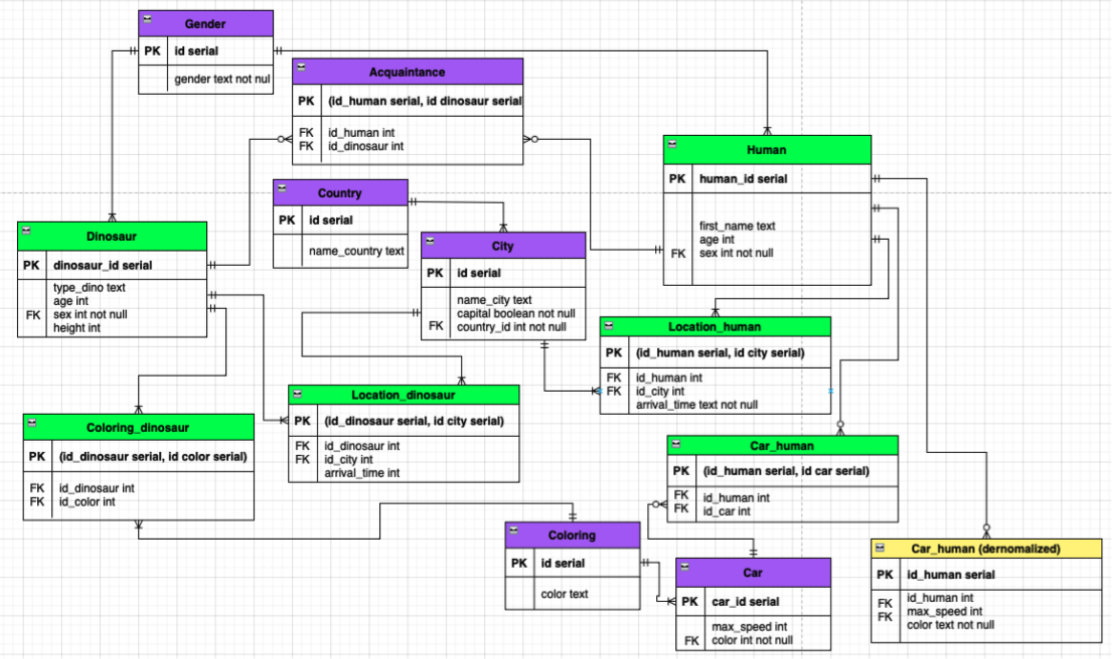
\includegraphics[width=.9\textwidth]{123}
\begin{lstlisting}[caption={kernel.ld}, label={lst:example}]
    
\end{lstlisting}
